\clearpage
\section{Lösungskonzept}\label{sec:Loesungskonzept}
\todo[inline]{Raffael}

Zur Messung und Auswertung der Mesh-Netzwerke dient ein Testframework, welches aus folgenden physikalisch getrennten Teilen besteht:

\begin{itemize}
	\item \textbf{TMS} Test Management Station \\ 
	Dient zur Verwaltung und Konfiguration des Testframeworks. Beinhaltet einen Webserver um dem Endanwender die Bedienung zu ermöglichen. Wird in der Aufgabenstellung (siehe \ref{app:Aufgabenstellung}) als Leitrechner bezeichnet. 
	\item \textbf{TMN} Test Management Node \\ 
	Dient als Zugangspunkt der im Testframework gefahrenen Tests und lässt sich über eine USB/UART Verbindung ansprechen. In der Aufgabenstellung (siehe \ref{app:Aufgabenstellung}) wird von einem Master gesprochen. 
	\item \textbf{FTN} Field Test Node \\ 
	Dient als Zugriffspunkt der im Testframework gefahrenen Tests und kann frei in der Testumgebung platziert werden. In der Aufgabenstellung (siehe \ref{app:Aufgabenstellung}) wird von einem Slave gesprochen. 
\end{itemize}

\begin{figure}[H]
	\centering
	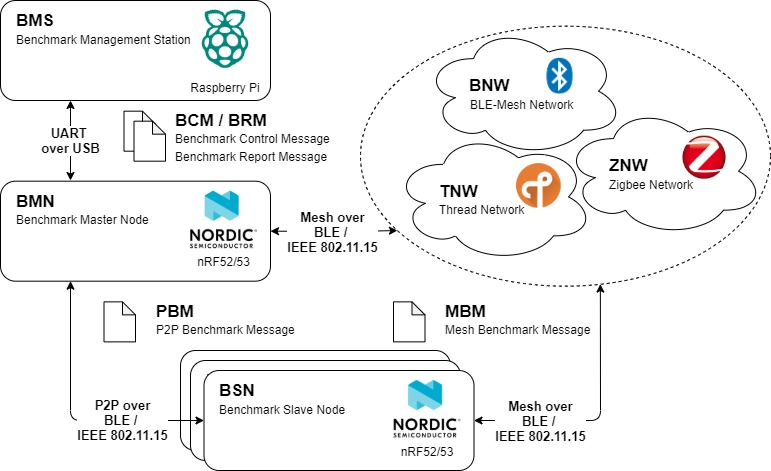
\includegraphics[width=1.0\textwidth]{Konzept_Testframework.jpg}
	\caption{Konzept Testfra4mework}\label{fig:KonzeptTestframework}
\end{figure}

\subsection{Punkt zu Punkt Testinfrastruktur}\label{subsec:PunktzuPunktTestinfrastruktur}
\todo[inline]{Raffael}


\subsection{Test Mesh Netzwerke}\label{subsec:TestMeshNetzwerke}

\subsubsection{Bluetooth Mesh}\label{subsubsection:Bluetooth Mesh}
\todo[inline]{Raffael}

\subsubsection{Thread}\label{subsubsection:Thread} 
\todo[inline]{Robin}

\subsubsection{Zigbee}\label{subsubsection:Zigbee}
\todo[inline]{Cyrill}


\subsection{Steuer und Auswertesoftware}\label{subsec:SteuerundAuswertesoftware}
\todo[inline]{Raffael}

